
\chapter{Especificação}\label{chp:espec}

\section{Arquitetura}

O sistema net.map precisa adquirir dados de potência dos sinais de redes \textit{Wi-Fi} para funcionar. Sendo assim, é necessário um dispositivo físico capaz de conseguir esses dados. Tendo em vista que os \textit{smartphones} possuem a capacidade de ler informações sobre as redes \textit{Wi-Fi} no ambiente ao seu redor, se tornam o dispositivo perfeito tanto para fazerem o mapeamento do ambiente quanto para ser utilizado pelo usuário final.\\
Tendo isso em mente, foi desenvolvido um aplicativo para dispositivos Android capaz de mapear ambientes e de verificar a localização atual. Esse \textit{app} se comunica com uma API rodando em um servidor na nuvem, responsável por fazer processamento dos dados utilizando algoritmos de \textit{Machine Learning}. Após processados, o resultado solicitado pelo usuário é retornado ao seu \textit{smartphone Android}.\\
O diagrama a seguir ilustra bem a arquitetura básica do sistema:

\begin{figure}[H]
	\centering
	\caption{Arquitetura do Sistema net.map}
  \includegraphics[width=0.8\textwidth]{diagramaArquitetura}
\label{fig:diagramaArquitetura}
\end{figure}


\section{Requisitos}\label{sec:req}

\subsection{Requisitos Funcionais}

\subsubsection{Aplicativo}
- Enviar dados sobre a intensidade dos sinais de \textit{Wi-Fi} ao servidor. \par
- Retornar a posição do usuário baseado nos dados enviados.\par
- O usuário deve inserir seu usuário e senha para poder usar o serviço.
\subsubsection{Servidor}
- A API deve funcionar não apenas com o aplicativo, mas com qualquer outra aplicação que utilize o protocolo HTTP.\par
- A API deve receber dados no formato JSON.\par
- Cada \textit{Facility} deve ter ao menos 2 zonas.\par
- Cada Zona deve ter ao menos 4 medidas.\par


\subsection{Requisitos Não-Funcionais}

\subsubsection{Aplicativo}
- O usuário deve ter um \textit{smartphone Android} com pelo menos a versão 4.1 instalada, além do aplicativo net.map.\par
\subsubsection{Servidor}
- A API deve ser transparente ao usuário.\par
- O usuário deve solicitar ao administrador do sistema um login e senha.\par



\section{Casos de Uso}

\subsection{Captura e Treinamento}

No primeiro caso de uso do sistema net.map, temos um usuário desejando mapear uma certa \textbf{instalação} (\textit{facility}, como é chamada no sistema). Ele deve planejar um mapa dividindo a instalação em seções menores, chamadas de \textbf{zonas}. Exemplo:

\begin{table}[htb]
\centering
\caption{Exemplo de divisão de instalação em zonas}
\label{my-label}
\begin{tabular}{|l|l|l|l|l|}
\hline
\multicolumn{5}{|c|}{\textbf{Instalação: Museu Paulista da USP}}             \\ \hline
\multicolumn{2}{|l|}{\textbf{Zona 1}} & \multicolumn{3}{l|}{Saguão de entrada}          \\ \hline
\multicolumn{2}{|l|}{\textbf{Zona 2}} & \multicolumn{3}{l|}{Exposição sobre Dom Pedro I}          \\ \hline
\multicolumn{2}{|l|}{\textbf{Zona 3}} & \multicolumn{3}{l|}{Sala do quadro \textit{Independência ou Morte}}          \\ \hline
\multicolumn{2}{|l|}{\textbf{Zona 4}} & \multicolumn{3}{l|}{Exposição sobre maquinário agrícola do séc. XIX}          \\ \hline
\multicolumn{5}{|c|}{\ldots}                                                    \\ \hline
\multicolumn{2}{|l|}{\textbf{Zona n}} & \multicolumn{3}{l|}{Exposição x}     \\ \hline
\end{tabular}
\end{table}

As zonas idealmente são melhores definidas como salas separadas por divisões físicas, tais como paredes ou andares. O confinamento dos sinais eletromagnéticos e a atenuação desses sinais ao atravessar paredes garante um resultado mais preciso. Porém, é possível delimitar linhas imaginárias para essas zonas, podendo demarcar zonas em grandes áreas sem paredes. O ideal é que essas zonas tenham uma área maior, garantido assim um resultado preciso.
\par
Após demarcar as zonas, é necessário configurar alguns parâmetros no aplicativo: número de aquisições por ponto e método de normalização.

\paragraph{Número de aquisições por ponto\\}
Para mapear uma zona, andamos por ela com o aplicativo de celular aberto, escaneando pontos discretos dentro dela. Como a potência do sinal das redes \textit{Wi-fi} é muito flutuante, o ideal é fazer uma média de várias aquisições para normalizar o valor lido naquele ponto. Isso é feito automaticamente pelo aplicativo.

\paragraph{Método de normalização\\}
Conforme explicado no parágrafo acima, é necessário normalizar os dados adquiridos devido à flutuação da potência de sinal. Esses dados podem ser normalizados através de uma média aritmética simples ou através de um método matemático chamado \textbf{Filtro de Kalman}. Este último será detalhado mais a frente. Um comparativo dos dois existe no capítulo 6.
\par

Terminando a configuração, é necessário percorrer a zona desejada, fazendo aquisições em pontos discretos dentro da zona. Idealmente, quantos mais pontos são capturados, melhor é a precisão da resposta final do sistema.

\subsection{Localização}
O modo de localização de usuário interage com a API instalada no servidor em nuvem, podendo assim ser implementado em qualquer dispositivo capaz de receber sinais \textit{Wi-Fi}. Utilizando uma aplicação que se comunica com a API, o usuário recebe a localização do servidor a cada novo escaneamento que é feito pela aplicação.

\section{Modelo de classes}
Como neste projeto utilizamos o MongoDB (banco de dados não-relacional orientado a documentos JSON), o conceito de entidade-relacionamento existente em bancos de dados SQL não faz muito sentido.
\par
Uma boa maneira de representar quais dados persistentes fazem parte do projeto é gerar um diagrama de classes da API no servidor:
\begin{figure}[H]
	\centering
	\caption{Diagrama das classes na API}
  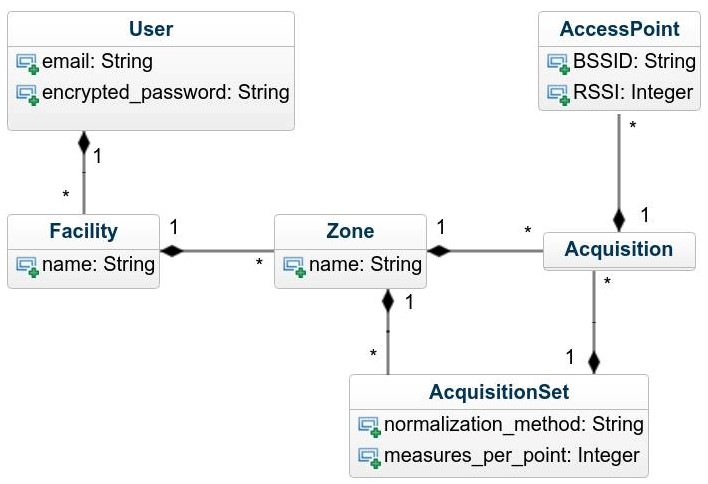
\includegraphics[width=0.8\textwidth]{classDiagram}
\label{fig:diagramaClasse}
\end{figure}


